\section{Motivation}

\logo{}

\begin{frame}{Forecast combination - point and density}

    Combining multiple forecasts can dramatically improve the accuracy of the forecast (\cite{BG69}).
    
    \vspace{5mm}

    
    Point Combination 
    \[y_t = \omega \ y_{1t} + (1-\omega) \ y_{2t}\]

    Density Combination
    \[f(y_t) = \omega \ f_1(y_t) + (1-\omega) f_2(y_t)\]


\begin{figure}[b]
\centering

\includegraphics[width=3cm]{Graph/Weather.jpg}
\end{figure}

\end{frame}


\begin{frame}{Forecast combination puzzle}

\begin{columns}[t]
    \begin{column}{0.5\textwidth}
        \centering
        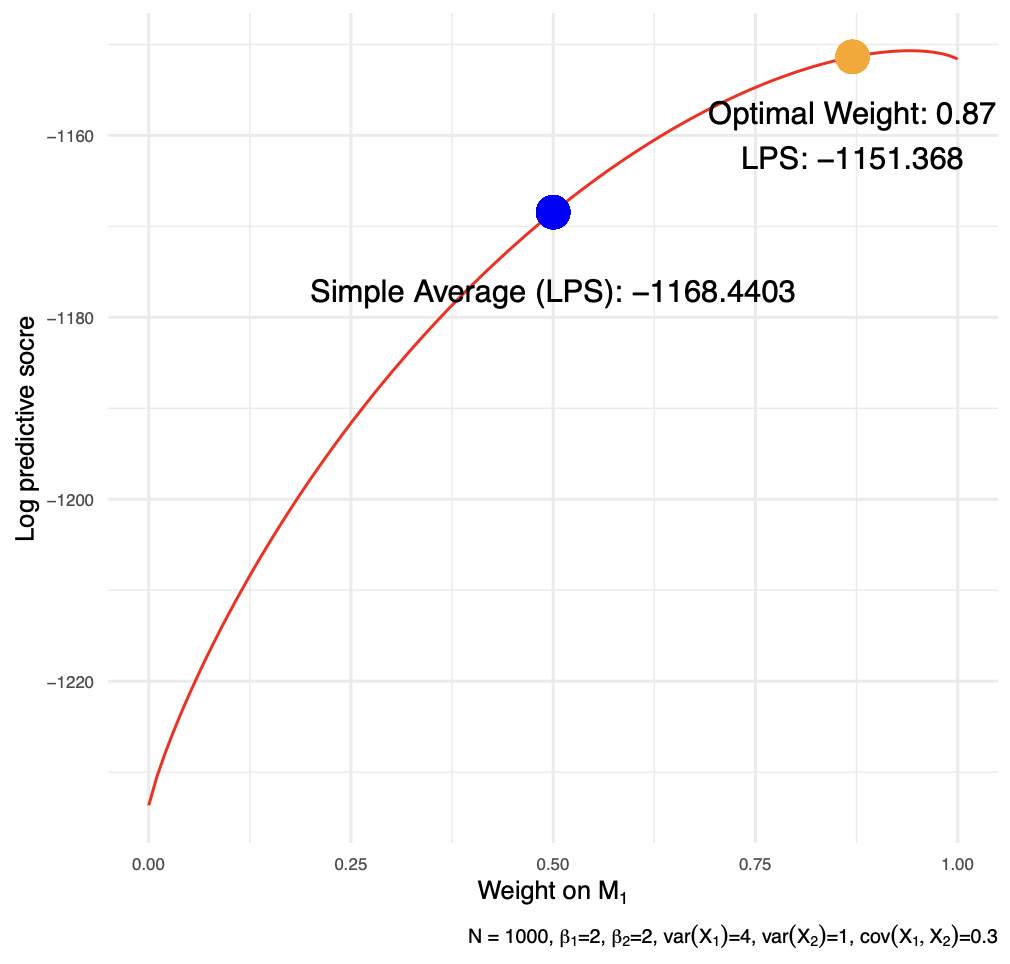
\includegraphics[width=6cm]{Graph/Ex1.png}
    \end{column}
    
    \begin{column}{0.5\textwidth}
        \centering
        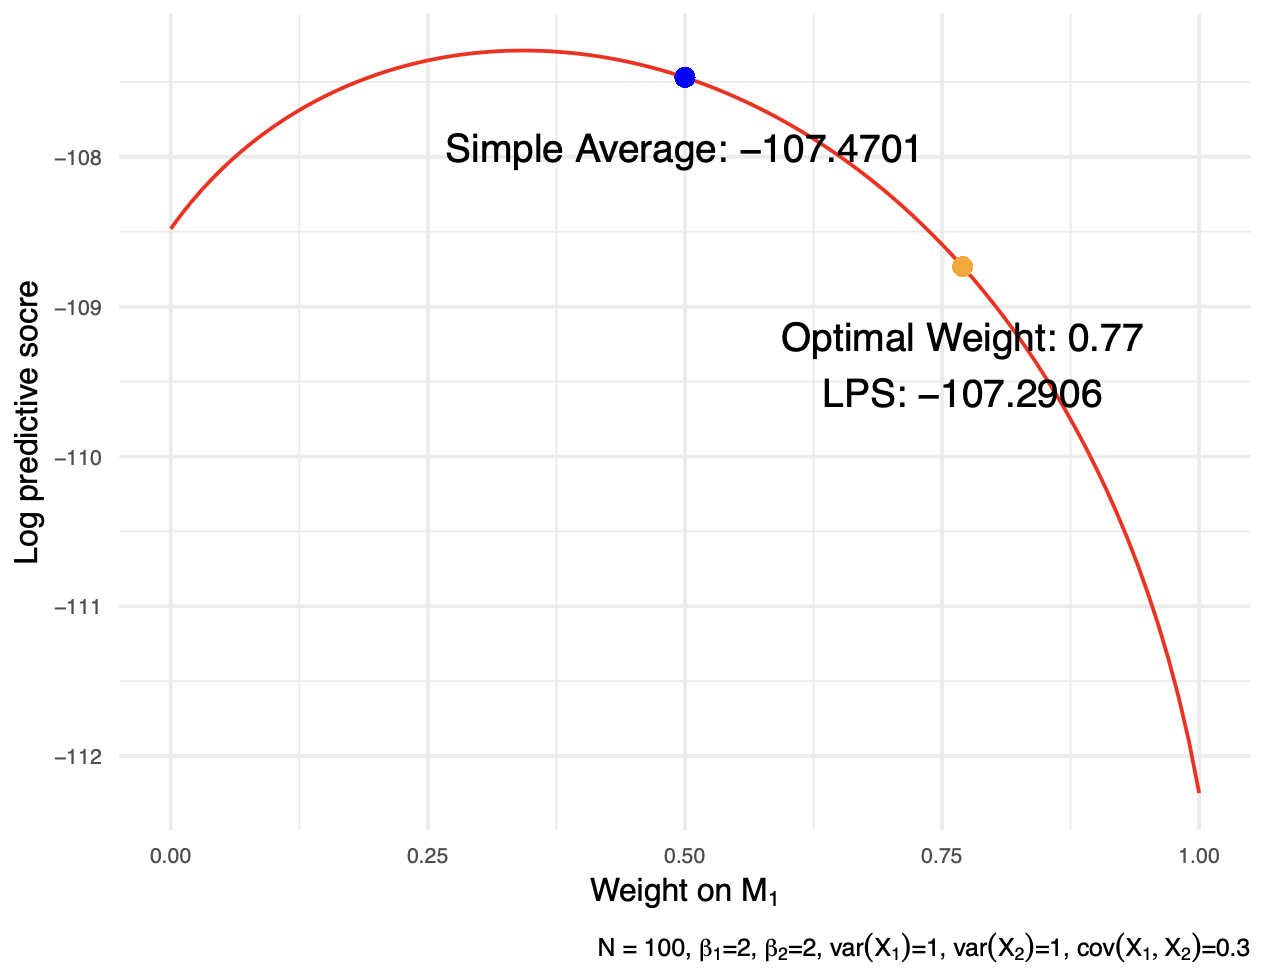
\includegraphics[width=6cm]{Graph/Ex2.png}
    \end{column}
    \end{columns}


    \begin{columns}[t]
    \begin{column}{0.5\textwidth}
        \begin{alertblock}{}
        \centering
        Complicated Weighting Schemes
        \end{alertblock}
    \end{column}
    
    \begin{column}{0.5\textwidth}
        \begin{exampleblock}{}
        \centering
        Simple Averaging
        / Equal Weights
        \end{exampleblock}
    \end{column}
    \end{columns}

\end{frame}



\begin{frame}{When should we expect the puzzle}

    In the linear regression context, the optimal weight $\hat\omega_{opt}$ has a closed-form expression when using the Mean Squared Error (MSE) weighting scheme.
    
    
    \[\hat\omega_{opt} \overset{p}{\to} \omega_\star = \frac{\alpha_1'\Sigma_{11}\alpha_1 - \alpha_1'\Sigma_{12}\alpha_2}{\alpha_1'\Sigma_{11}\alpha_1 - 2\alpha_1'\Sigma_{12}\alpha_2 + \alpha_2'\Sigma_{22}\alpha_2}\]


    The presence of the puzzle is highly relevant to the coefficients and the variances of regressors in both models.
    
    
    \[\omega_\star=\frac{1}{2} \Rightarrow \alpha_1'\Sigma_{11}\alpha_1 = \alpha_2'\Sigma_{22}\alpha_2\]

    In-sample performance

    
\end{frame}




\begin{frame}{Preliminary Conjecture}

    Consider a simple case of two-model combination.

    \begin{table}[ht]
    \centering
    \begin{tabular}{cccc}
                           &      & \multicolumn{2}{c}{$M_2$} \\
                           &      & Good       & Bad       \\
    \multirow{2}{*}{$M_1$} & Good & $\surd$    & $?$ \\
                           & Bad  & $?$        & $\surd$
    \end{tabular}
    \label{tab:1}
    \caption{Initial conjecture on the presence of forecast combination puzzles when combining two models}
    \end{table}
    
    \hspace*{20pt} The in-sample fit comparison between two models 
    
    \hspace*{20pt} The presence of the puzzle


\end{frame}


\begin{frame}{Preliminary Conjecture}

\begin{figure}
    \centering
    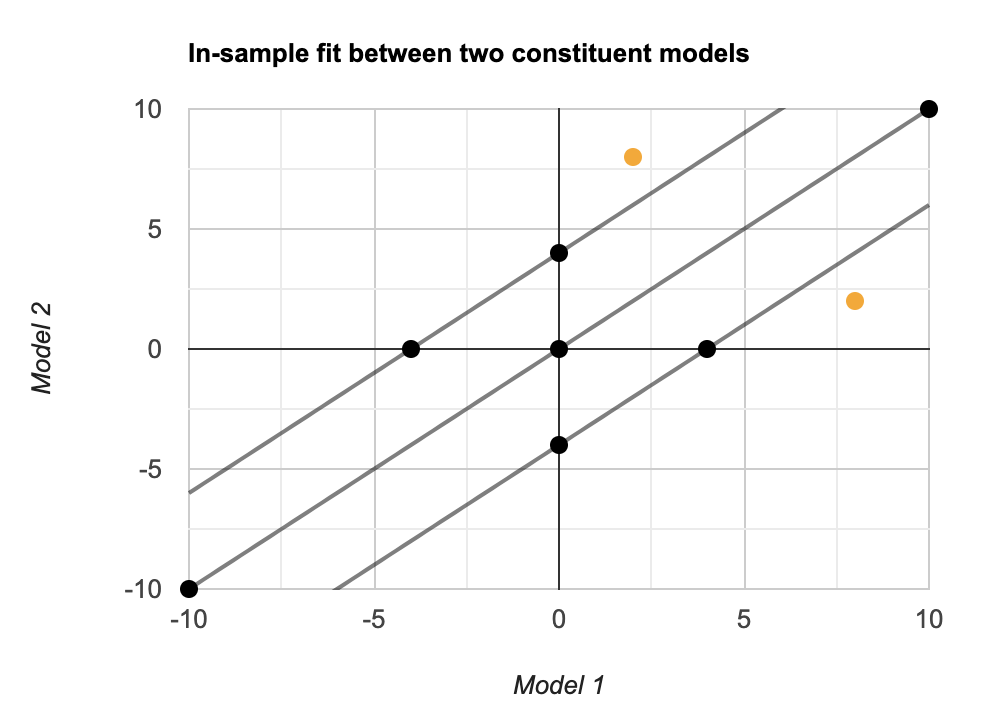
\includegraphics[width=8cm]{Graph/Conjecture.png}
    \label{fig:enter-label}
\end{figure}


\end{frame}





